\begin{questions}
\question{
Reciprocal basis 2D}
\begin{solution}
  To tackle this problem it is useful to remember the following relation between the vectors of the direct and reciprocal basis
  \begin{equation}
    \vec{a}_i\cdot \vec{b}_j = 2\pi \delta_{ij}.
  \end{equation}
  Now if we take vectors in two dimensions, this yields the following matrix equation
  \begin{equation}
    \begin{pmatrix}
      b_{1x} & b_{1y}\\
      b_{2x} & b_{2y}
    \end{pmatrix}
    \begin{pmatrix}
      a_{1x} & a_{2x}\\
      a_{1y} & a_{2y}
    \end{pmatrix}
    = 2\pi \begin{pmatrix}
      1 &0\\
      0 & 1
    \end{pmatrix}.
  \end{equation}
  If we solve the equation for $\mathcal{B}$ then we have
  \begin{equation}
    \begin{pmatrix}
      b_{1x} & b_{1y}\\
      b_{2x} & b_{2y}
    \end{pmatrix}
    = \frac{2\pi}{a_{1x}a_{2y} - a_{1y}a_{2x}} \begin{pmatrix}
      a_{2y} & -a_{2x}\\
      -a_{1y} & a_{1x}
    \end{pmatrix}.
  \end{equation}
  The vectors given in the assignment for the direct basis give us the matrix $\mathcal{A}$
  \begin{equation}
    \mathcal{A}
    =  \begin{pmatrix}
      a & a/2\\
      0 & a
    \end{pmatrix},
  \end{equation}
  therefore
  \begin{equation}
    \begin{pmatrix}
      b_{1x} & b_{1y}\\
      b_{2x} & b_{2y}
    \end{pmatrix}
    = \frac{2\pi}{a^2} \begin{pmatrix}
      a & -a/2\\
      0 & a
    \end{pmatrix} = \begin{pmatrix}
      2\pi/a & -\pi/a\\
      0 & 2\pi/a
    \end{pmatrix}.
  \end{equation}
  Hence, the primitive vectors of the reciprocal lattice are
  \begin{eqnarray}
    \vec{b}_1 =\begin{pmatrix}
      2\pi/a\\
      0
    \end{pmatrix}, \quad \vec{b}_2 = \begin{pmatrix}
       -\pi/a\\
       2\pi/a
    \end{pmatrix}.
  \end{eqnarray}
  The respective drawings of the first and second Brillouin zones can be seen in fig. \ref{brill}
  \begin{center}
    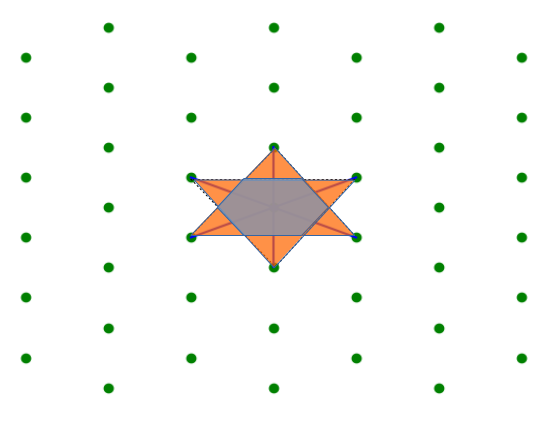
\includegraphics[width=65mm]{brill}
  \end{center}
  \captionof{figure}{First (hexagon) and second (star) Brillouin zones.}\label{brill}\vspace{0.5cm}
\end{solution}

\question{Areas of the Brillouin zones}
\begin{solution}
  First we need to remember that all Brillouin zones have the same area. Then we only need to calculate the area of the first one. From fig. \ref{brill} we can see that the length apothem is half of the size of the vector $(2\pi/a, 0)$, that is $ap = \pi/a$. Now, by doing simple trigonometry and recalling that all the triangles inside the hexagon are equilateral, since it is a regular hexagon,   we will have that the length of each side of the hexagon is equal to $b=2ap/\sqrt{3}$. This result comes as a consequence of Pythagoras theorem. Finally, if we remember that the area of an hexagon is $6*b*ap/2$ we find
  \begin{equation}
    A = \frac{6b(ap)}{2} =  \frac{6(ap)^2}{\sqrt{3}} =  \frac{2(\sqrt{3})^2\pi^2}{a^2\sqrt{3}} = \hlgreen{\frac{2\sqrt{3}\pi^2}{a^2}.}
  \end{equation}
\end{solution}

\end{questions}

%
% \begin{center}
%   \includegraphics[width=55mm]{}
% \end{center}
%
% \captionof{figure}{}\label{new}\vspace{0.5cm}
